%%%%%%%%%%%%%%%%%%%%%%%%%%%%%%%%%%%%%%%%%%%%%%%%%%%%%%%%%%%%%%%%%%%%%%%%%%%%%%%%
%2345678901234567890123456789012345678901234567890123456789012345678901234567890
%        1         2         3         4         5         6         7         8

\documentclass[letterpaper, 10 pt, conference]{ieeeconf}
\IEEEoverridecommandlockouts
\overrideIEEEmargins
\usepackage{cite}
\usepackage{amsmath,amssymb,amsfonts,amsthm,color,float}
\usepackage{algorithmic}
\usepackage{graphicx}
\usepackage{textcomp}
 \usepackage{calc}
 \usepackage{tikz}
\usepackage{cases}
\usepackage{verbatim}
\usepackage{hyperref}
\usepackage{xcolor, soul}
\usepackage{mathtools, nccmath}

\theoremstyle{plain}
\newtheorem{thm}{Theorem}
\newtheorem{cor}{Corollary}
\newtheorem{prop}{Proposition}
\newtheorem{conj}{Conjecture}
\newtheorem{lemma}{Lemma}
\newtheorem{claim}{Claim}

\theoremstyle{definition}
\newtheorem{defn}{Definition}
\newtheorem{assum}{Assumption}
\newtheorem{ex}{Example}
\newtheorem*{rem*}{Remark}

\theoremstyle{remark}
\newtheorem{obs}{Observation}


% general math notation
\renewcommand{\rm}[1]{\mathrm{#1}}
\newcommand{\bb}[1]{\mathbb{#1}}
\newcommand{\cl}[1]{\mathcal{#1}}
\newcommand{\R}{\bb{R}}
\newcommand{\N}{\bb{N}}



\begin{document}
\title{Learning Efficient Strategies in Resource Utilization with Degradation}
\author{Bryce L. Ferguson and Rohit Konda}

\maketitle
\thispagestyle{empty}

The main thesis of this research proposal is on the design and analysis of adaptive algorithms that dictate utilization of resources in a dynamical setting. Distinctive to this setting is that when a resource is increasingly utilized, its current operating quality degrades further, and thus effective algorithms must manage this fundamental trade-off. As such, providing good algorithms in this framework has deep implications in various application domains. For example, consider rider-sharing platforms; these services have become ubiquitous, and so operating these platforms in an efficient manner is vital for rider satisfaction and minimizing usage costs. This setting also inherits this fundamental trade-off from the following perspective. Drivers span through areas of an urban landscape depending on the present rider demand. Rider demand (number of un-serviced riders) in areas that are serviced by drivers are expected to decrease while areas that are not serviced are expected to accumulate a surplus of rider demand. Managing this fundamental trade-off appear in various other application domains as well, including 






First, consider when drivers are traveling across areas of an urban landscape. When drivers operate in a specific area, some riders will be serviced, and the demand decreases. However, in areas that are not worked by active drivers, the number of un-serviced riders (and thus, demand) will increase. In this way, the goal of the driving-fleet operator is to allocate drivers across many locations with the objective of minimizing the total number waiting drivers.

Attaining this goal will take many steps, including deriving the optimal policy for allocating drivers that considers the dynamic and adaptive demand as well as implementing these policies in a feasible way.

Our proposed research will aid in these two challenges in urban transit design, but will also serve purpose in several disparate areas with degradable resources, such as battery power storage/utilization, server queuing, task-assignment, renewable energy sources, and more.

With this in mind, we propose the study of a general dynamic resource allocation problem in which a resource's value degrades as it is utilized.
The general framework will allow our results to provide relevant insights to several problem domains.
We take inspiration from \emph{fishery games} that were studied in the economics literature in the 1980's, where the emphasis  was on protecting a common good from a social policy perspective. In our work, we take an novel outlook on this model: considering the designed utilization in engineered settings.
This new perspective offers new opportunities for applying relevant tools but also new challenges presented by the engineering problem domains.

More formally, we consider a set of resources to be utilized by a set of agents. These agents can select (or be assigned) resources to utilize at different points in time; the agents generate value or benefit from accessing these resources. However, the utilization of a resource can affect its quality or availability in the future (e.g., farming fish from a lake today means less fish in that lake tomorrow). In this sense, greedy utilization in the short term by agents can lead to deficiencies in the long-term. To the agents and the operator, there exists a natural trade-off, in which they must balance short and long-term gains when utilizing resources.
This trade-off is precisely what we seek to analyze.
In this pursuit, several important and interesting questions emerge:


\begin{figure}
    \centering
    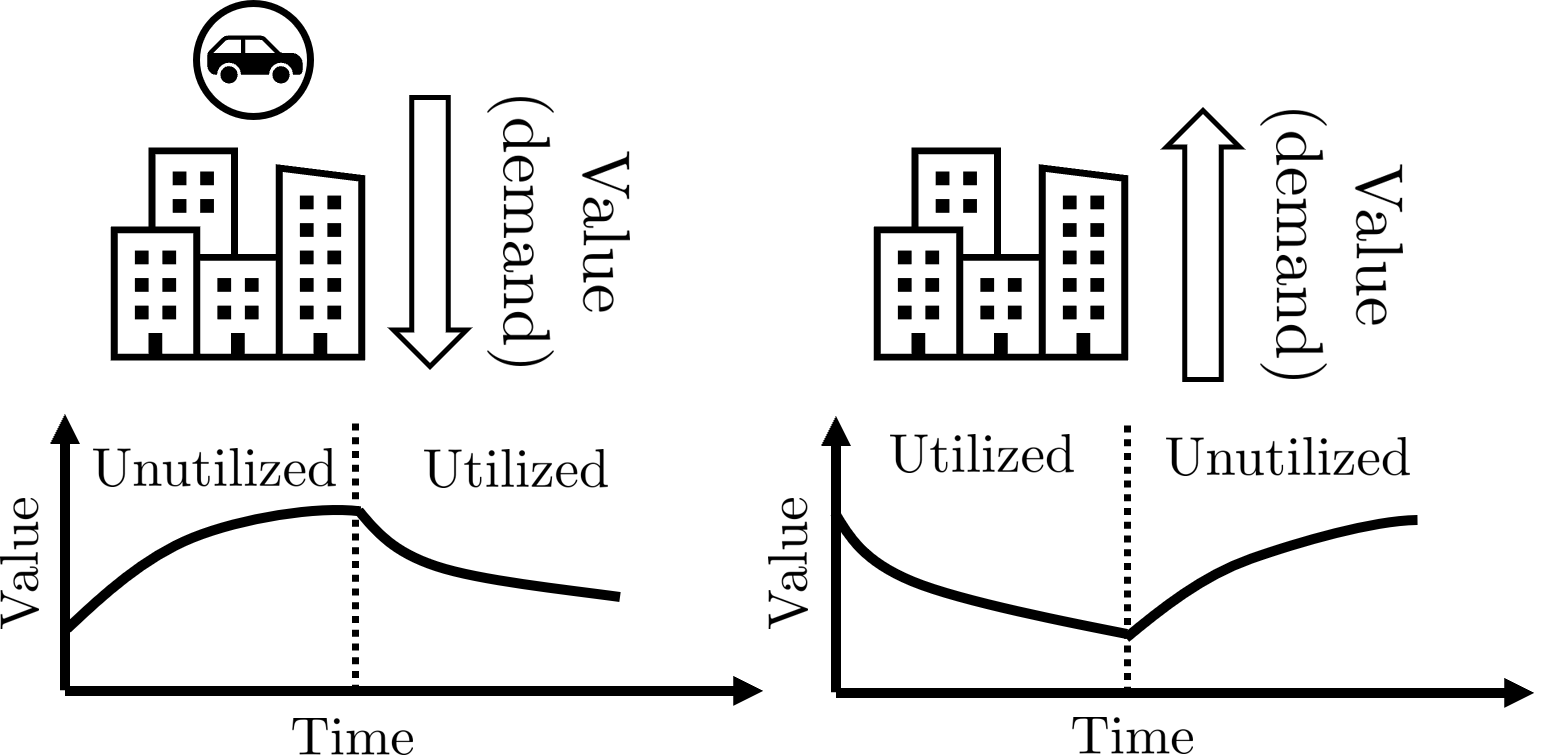
\includegraphics[width=\columnwidth]{fig_city_2.png}
    \caption{An illustration of a neighborhood (resource) being serviced (utilized) by urban transit vehicles (agents). While an area is being serviced, the demand (or value) of the region is depleted. While an area is non serviced, the demand rises. A successful operator such a system will consider the affect of these dynamics in their resource allocation.}
    \label{fig:app}
    \vspace{-5mm}
\end{figure}

\noindent\textit{- How do we optimally utilize resources which are affected by our actions?} As a resource is utilized, its future value degrades. As it is left unutilized, its future value grows. How does a system operator optimize the long run value extracted from this resource by alternating times of utilization and rest?

\noindent\textit{- What impact does decentralized decision making have on the system?} In some settings, the system operator may not have the ability to directly assign actions to each agent (e.g., ride-sharing with human drivers). However, they are able to design objectives for each agent to evaluate locally (e.g., pricing schemes). How does this local/decentralized decision making affect the overall system performance?

\noindent\textit{- How does uncertainty in a resources future value affect design and performance?} Resources may not degrade deterministically, an agent's utilization may have random or uncertain consequences on the resources value. How can the system operator learn this behavior and optimize around it?

\noindent\textit{- How do restrictions on agent decisions impact resource utilitization?} When agents are restricted in the resources they can utilize, or even heterogeneous, (e.g., drivers only working certain areas), then how does a system operator optimize around these constraints?


The way that we solve these question is through analysis via control theory and reinforcement learning. 
The innovation our proposal brings is the application of controls and learning to a framework with relevant features to many engineered problems, but has yet to be adapted to this setting.



\end{document}


For example, a battery management system may have access to several power storage devices, such as the proposed ideas of vehicle-to-grid charging where EV batteries can be used to store and supply power to a local grid. As a battery is used, its charge is depleted making it less valuable as a power source; further, in the case of the vehicle-to-grid charging scheme, it becomes less valuable as a car power supply. We can also model security problems in this framework.  Additionally, we can examine problems of dynamic server queing, natural resource harvesting, and task assignment from this framework.

These examples both highlight the fact that resource allocation/utilization is a dynamic process and effectively utilizing resources means adaptively changing how resources are allocated. Deriving algorithms which optimally utilize degradable resources will prove valuable in improving the operation of complex systems